\documentclass[tikz,border=6pt]{standalone}

\usepackage{pgfplots}
\pgfplotsset{compat=1.18}

\begin{document}
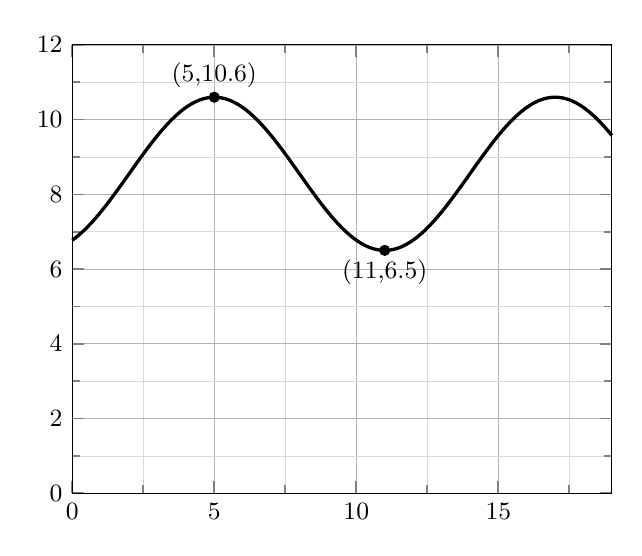
\begin{tikzpicture}
\begin{axis}[
%   width=12.5cm,
%   height=6.2cm,
  xmin=0, xmax=19,
  ymin=0, ymax=12,
  axis lines=box,
  grid=both,
  major grid style={line width=0.3pt, draw=gray!60},
  minor grid style={line width=0.2pt, draw=gray!30},
  minor tick num=1,
  xtick={0,5,10,15,20},
  ytick={0,2,4,6,8,10,12},
  tick style={line width=0.6pt},
  ticklabel style={font=\small},
  clip=false
]

% Model from the data: midline 8.55, amplitude 2.05, period 12, max at t=5
\addplot[
  domain=0:19,
  samples=300,
  smooth,
  very thick
] {8.55 + 2.05*cos(30*(x-5))};

% Marked points
\addplot[only marks, mark=*, mark size=1.8pt] coordinates {(5,10.6) (11,6.5)};

\node[font=\small, above] at (axis cs:5,10.6) {(5,10.6)};
\node[font=\small, below] at (axis cs:11,6.5) {(11,6.5)};

\end{axis}
\end{tikzpicture}
\end{document}
